\section{Results and Discussion}\label{sec:evaluation}
% In the ENMU Computer Science program, CSCI 1210: the Computer Programming Fundamentals course is taught in Java and delivered in a hybrid format, combining in-person instruction with asynchronous distance learning. To evaluate \codeinspectoren, students were assigned a benchmark task that required them to implement a method that converts the rank and suit of a playing card from shorthand notation to its complete descriptive form. A total of 19 submissions, comprising 1,315 lines of code, were submitted to \codeinspector to assess code quality and correctness, with a copy of each assessment result automatically emailed to the corresponding student.

% \begin{figure}
%     \centering
%     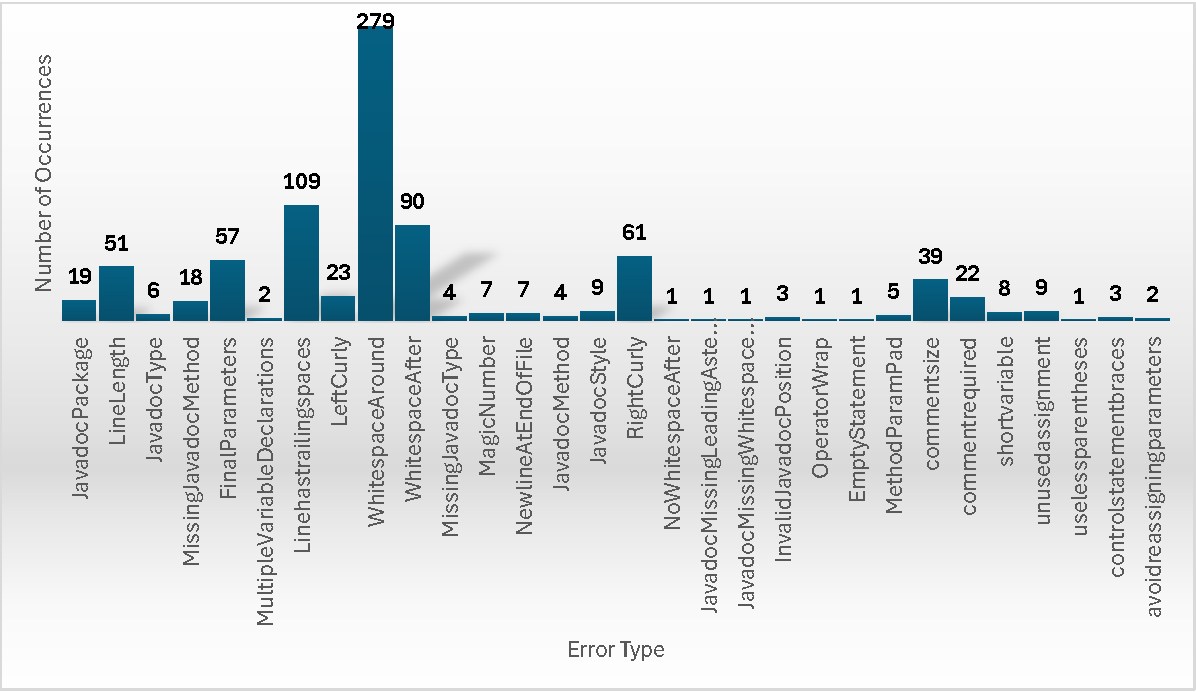
\includegraphics[width=\linewidth]{fig/style_err_freq.pdf}
%     \caption{Frequency distribution of detected style errors.}
%     \label{fig:style_errors}
% \end{figure}

% Figure~\ref{fig:style_errors} shows the frequency of coding standards violations identified by CheckStyle and PMD within \codeinspectoren, totaling 843 style errors. Of these, \textit{\quotes{WhiteSpaceAround,}} \textit{\quotes{LineHasTrailingSpaces,}} and \textit{\quotes{WhiteSpaceAfter}} were the most frequently occurring violations in all submissions. While whitespace errors do not affect code functionality, they reduce code readability and hinder collaboration, making it harder for reviewers to understand changes during code reviews and maintenance.

% \begin{figure}
%     \centering
%     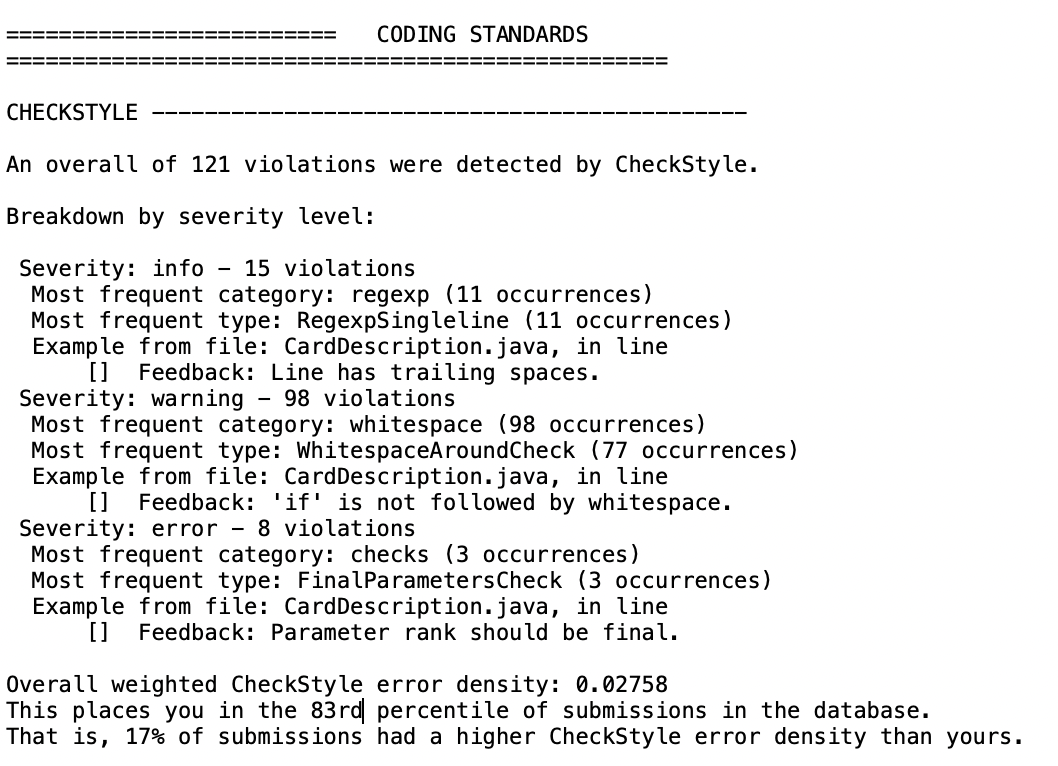
\includegraphics[width=0.93\linewidth]{fig/feedback_style.png}
%     \caption{Style errors detected by CheckStyle.}
%     \label{fig:CheckStyle_results}
% \end{figure}

% Figure~\ref{fig:CheckStyle_results} presents a portion of a report generated by \codeinspector for a student's code submission, showing style errors detected by CheckStyle. Due to space limitations, violations identified by PMD are omitted. Of the 121 errors reported by CheckStyle, 15 were classified as \quotes{info,} 98 as \quotes{warning,} and eight as \quotes{error,} highlighting issues that range from minor suggestions to critical problems requiring immediate attention. Notably, the most frequent violations across all categories were \textit{\quotes{WhiteSpaceAround}} and \textit{\quotes{LineHasTrailingSpaces}} (88 occurrences), as well as \textit{\quotes{FinalParametersCheck}} (3 occurrences), which highlights a recurring pattern of non-final parameters in methods, a common pitfall in early-stage programming education. This report demonstrates the system's ability to provide granular and actionable feedback, enabling students to identify areas for stylistic improvement and iteratively refine their code based on clear, rule-based guidelines. Additionally, the report's structured breakdown by severity and category enables instructors to prioritize feedback.

% \codeinspectoren's integration of CheckStyle further demonstrates its utility in contextualizing student performance. For example, the reported error-weighted density (0.02758) places this submission in the 83rd percentile of analyzed submissions, indicating a higher rate of code style violations than 83\% of the sumissions, reflecting weaker adherence to coding standards. This comparative metric underscores the system's ability to deliver formative feedback and benchmarking insights, fostering self-awareness and motivating continuous improvement. Such automated, data-driven assessments also reduce instructors' grading burdens while ensuring consistent and objective evaluation, which is a critical step toward scalable, high-quality coding education.

% \begin{figure}[h]
%     \centering
%     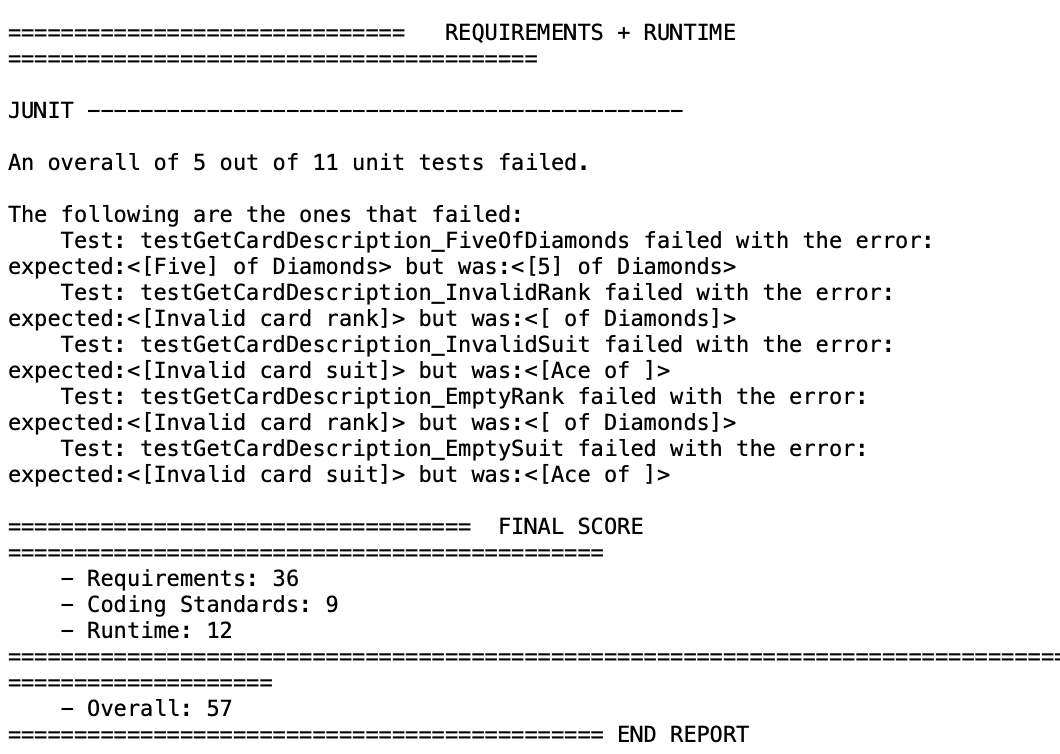
\includegraphics[width=0.93\linewidth]{fig/feedback_req.png}
%     \caption{Unit testing results and final scores from the generated feedback.}
%     \label{fig:Grade_report}
% \end{figure}

% Figure 4 presents another portion of the same feedback report shown in Figure~\ref{fig:CheckStyle_results}, highlighting formative feedback generated by \codeinspector to help students address functional issues in their code. The report demonstrates the effectiveness of \codeinspectoren's automated testing framework powered by JUnit and LLM-generated test cases in identifying correctness issues and assigning holistic scores to student submissions. For this particular submission, 11 unit test cases were executed, of which six passed successfully, while five failed due to various issues detailed in the feedback. One such issue involved a discrepancy between the expected output string (\quotes{[Five] of Diamonds}) and the actual output (\quotes{[5] of Diamonds}). This granular feedback exemplifies how \codeinspector leverages LLM-driven test generation to pinpoint logical errors, enabling students to refine their code against precise, real-world expectations iteratively.

% Moreover, the final score breakdown further underscores \codeinspectoren's modular evaluation design, which balances multiple assessment criteria (e.g., requirements fulfillment, coding standards, runtime performance) to reflect holistic competency. For this particular submission, \codeinspector assigned an overall score of 57, demonstrating its ability to synthesize diverse evaluative dimensions into actionable insights. This structured, automated scoring mechanism streamlines grading while ensuring transparency and consistency, aligning with pedagogical goals of fostering technical rigor and supporting iterative improvement in student work.